\documentclass[11pt,a4paper]{article}

\usepackage[T1]{fontenc}
\usepackage[utf8]{inputenc}
\usepackage{lmodern}
\usepackage[a4paper,margin=1in]{geometry}
\usepackage{amsmath,amssymb,amsthm,mathtools,bm}
\usepackage{physics}
\usepackage{graphicx}
\usepackage{booktabs}
\usepackage{microtype}
\usepackage{xcolor}
\usepackage{hyperref}
\usepackage{enumitem}
\usepackage{tikz}
\usetikzlibrary{arrows.meta,calc,positioning,decorations.pathmorphing,decorations.pathreplacing}

\hypersetup{
  colorlinks=true,
  linkcolor=blue!60!black,
  citecolor=blue!60!black,
  urlcolor=blue!60!black
}

\setlength{\parskip}{0.45em}
\setlength{\parindent}{0pt}
\setlist[itemize]{leftmargin=1.4em}
\setlist[enumerate]{leftmargin=1.6em}

\newtheorem{proposition}{Proposition}
\newtheorem{remark}{Remark}

\title{Delayed Mode Selection and Parity-Separated Observables in a Rapidly Rotating Fluid Column with Event-Triggered Reinjection}
\author{Omar Iskandarani\\
\small Independent Researcher, Groningen, The Netherlands\\
\small \href{mailto:info@omariskandarani.com}{info@omariskandarani.com}}
\date{Draft compiled on \today}

\begin{document}
\maketitle

\begin{abstract}
We study a classical rotating-fluid platform in which axisymmetric forcing, finite axial transport time, and event-triggered reinjection combine to form a delayed nonlinear loop. The starting point is a rapidly rotating cylindrical column driven by a bottom rotor under a steady background rotation. In the low-Rossby, low-Ekman regime, axisymmetric vertical forcing generates a delayed axial response governed by rotating-fluid transport rather than instantaneous communication. We show how this delayed transport can be converted into a regenerative feedback loop by triggering each subsequent rotor pulse from a detected surface event after a prescribed digital latency.

Two distinct observable sectors are then naturally separated by parity. The first is an odd sector, represented by signed azimuthal or angle-like response variables, which reverses under reversal of the axial forcing sign. The second is an even sector, represented by scalar response measures quadratic in velocity or swirl amplitude, which remain invariant under sign reversal. This parity split implies that a symmetric up/down forcing protocol can exhibit leading-order cancellation in the odd sector while retaining a nonzero accumulated contribution in the even sector.

To connect the fluid platform to delayed nonlinear dynamics, we formulate a reduced event-triggered loop model with effective delay $\tau_{\mathrm{eff}}$ and gain $\kappa_{\mathrm{eff}}$. In the reinjected regime, the platform becomes a classical delayed-feedback system admitting mode selection, branch survival, multistability, and transition to irregular dynamics as the effective gain-delay product is increased. We outline experimentally measurable criteria distinguishing one-pass delayed transport from genuine delayed-loop branch selection. The results require no quantum assumptions and identify a rotating-fluid route from finite propagation time to classical order, hysteresis, and chaos.
\end{abstract}

\section{Introduction}

Closed dynamical loops with finite propagation speed form a broad class of classical systems in which delay is not merely a correction to local dynamics, but a constitutive ingredient. In optical rings, electronic delay lines, and phase-locked feedback architectures, finite transit time can organize the dynamics into stable operating branches, multistable regimes, or irregular motion. Separately, rapidly rotating fluids support strongly anisotropic transport and wave propagation, with axial communication governed by rotation-induced structure rather than by the kinematics of non-rotating flow.

The present work combines these two themes in a single classical platform: a rapidly rotating cylindrical fluid column with axisymmetric forcing and event-triggered reinjection. The physical picture is simple. A bottom rotor, embedded in a slowly rotating cylinder, launches a disturbance into a rotation-prepared medium. Under suitable conditions the response is not dominated by immediate radial spreading, but by delayed axial transport toward the free surface. Once that delayed response is used to trigger a subsequent rotor pulse, the platform is promoted from a one-pass transport experiment to a regenerative delayed loop.

This permits two conceptually distinct questions to be addressed within one setup. The first is a rotating-fluid question: under what conditions does axisymmetric forcing generate a reproducible delayed axial response rather than a predominantly divergent radial disturbance? The second is a nonlinear-dynamical question: once the detected arrival event is fed back to the actuator, does the resulting loop display branch selection, multistability, or transitions to irregular dynamics as a function of effective delay and gain?

A second theme of the present paper is parity separation. In the same rotating-fluid platform, different observables transform differently under reversal of the sign of the axial forcing. Signed angle-like observables are odd under reversal, while scalar quadratic measures built from speed, swirl intensity, or response amplitude are even. This creates a structurally sharp possibility: a symmetric forcing protocol may exhibit cancellation in one observable sector while accumulating a nonzero signal in another. The point is classical and kinematic. No microscopic interpretation is required for the parity statement itself.

The goal of this paper is deliberately narrow. We do not claim a new constitutive law for matter, nor any modification of standard wave or fluid theory. Instead, we isolate a minimal classical mechanism,
\begin{equation}
\text{rotation} + \text{finite transport time} + \text{event-triggered reinjection}
\Longrightarrow
\text{delayed nonlinear loop dynamics},
\end{equation}
and identify a parity split,
\begin{equation}
\text{odd signed sector} \oplus \text{even scalar sector},
\end{equation}
within which delayed transport and reinjection create a platform for order, branch selection, hysteresis, and possibly chaos.

\begin{figure*}[t]
\centering
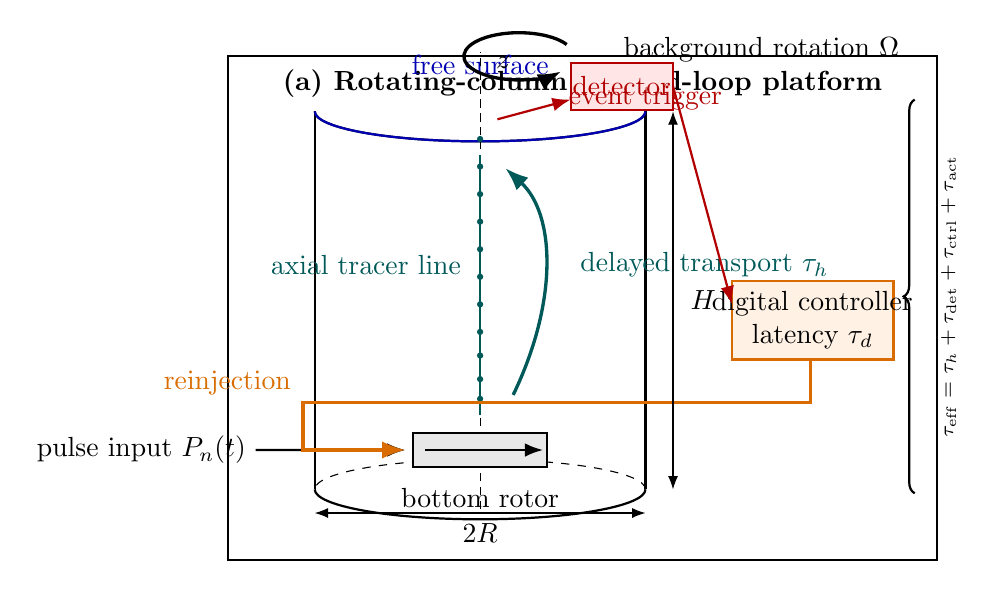
\begin{tikzpicture}[x=1cm,y=1cm,>=Latex]

% =========================================================
% PANEL (a): setup
% =========================================================
\begin{scope}[shift={(0,0)}]
  \draw[thick] (0,0) rectangle (9.0,6.4);
  \node[font=\bfseries] at (4.5,6.05) {(a) Rotating-column delayed-loop platform};

  % Cylinder geometry
  \def\R{2.1}
  \def\H{4.8}
  \def\ey{0.38}
  \coordinate (C0) at (3.2,0.9);

  % Cylinder
  \draw[thick] ($(C0)+(-\R,0)$) arc[start angle=180,end angle=360,x radius=\R,y radius=\ey];
  \draw[thick] ($(C0)+(-\R,\H)$) arc[start angle=180,end angle=360,x radius=\R,y radius=\ey];
  \draw[thick] ($(C0)+(-\R,0)$) -- ($(C0)+(-\R,\H)$);
  \draw[thick] ($(C0)+(\R,0)$) -- ($(C0)+(\R,\H)$);
  \draw[dashed] ($(C0)+(\R,0)$) arc[start angle=0,end angle=180,x radius=\R,y radius=\ey];

  % Free surface
  \draw[blue!70!black, thick] ($(C0)+(-\R,\H)$) arc[start angle=180,end angle=360,x radius=\R,y radius=\ey];
  \node[blue!70!black, above] at ($(C0)+(0,\H+0.35)$) {free surface};

  % z-axis
  \draw[densely dashed] ($(C0)+(0,-0.25)$) -- ($(C0)+(0,\H+0.75)$);
  \node[right] at ($(C0)+(0.08,\H+0.62)$) {$z$};

  % Background rotation
  \draw[->, very thick] ($(C0)+(1.1,\H+0.85)$) arc[start angle=30,end angle=320,x radius=0.7,y radius=0.30];
  \node[right] at ($(C0)+(1.7,\H+0.78)$) {background rotation $\Omega$};

  % Rotor
  \filldraw[fill=gray!18, draw=black, thick] ($(C0)+(-0.85,0.28)$) rectangle ($(C0)+(0.85,0.72)$);
  \draw[thick] ($(C0)+(-0.7,0.5)$) -- ($(C0)+(0.7,0.5)$);
  \draw[->, thick] ($(C0)+(0,0.5)$) -- ($(C0)+(0.8,0.5)$);
  \node[below] at ($(C0)+(0,0.14)$) {bottom rotor};

  % Input pulse
  \draw[->, thick] (0.35,1.4) -- ($(C0)+(-0.95,0.5)$);
  \node[left] at (0.35,1.4) {pulse input $P_n(t)$};

  % Central tracer line
  \draw[teal!70!black, line width=1.0pt] ($(C0)+(0,0.95)$) -- ($(C0)+(0,\H-0.55)$);
  \foreach \yy in {1.15,1.4,1.7,2.0,2.35,2.7,3.05,3.4,3.75,4.1,4.45} {
    \fill[teal!70!black] ($(C0)+(0,\yy)$) circle (0.04);
  }
  \node[teal!70!black, left] at ($(C0)+(-0.12,2.85)$) {axial tracer line};

  % Delayed transport arrow
  \draw[->, very thick, teal!70!black] ($(C0)+(0.42,1.2)$) .. controls ($(C0)+(1.0,2.4)$) and ($(C0)+(0.95,3.5)$) .. ($(C0)+(0.32,\H-0.72)$);
  \node[teal!70!black, right] at ($(C0)+(1.15,2.85)$) {delayed transport $\tau_h$};

  % Detector
  \filldraw[fill=red!10, draw=red!70!black, thick] ($(C0)+(1.15,\H+0.02)$) rectangle ($(C0)+(2.45,\H+0.62)$);
  \node[red!70!black] at ($(C0)+(1.8,\H+0.32)$) {detector};
  \draw[->, red!70!black, thick] ($(C0)+(0.22,\H-0.10)$) -- ($(C0)+(1.15,\H+0.15)$);

  % Controller
  \filldraw[fill=orange!10, draw=orange!85!black, thick] (6.4,2.55) rectangle (8.45,3.55);
  \node[align=center] at (7.42,3.05) {digital controller\\ latency $\tau_d$};

  % Detector to controller
  \draw[->, red!70!black, thick] ($(C0)+(2.45,\H+0.32)$) -- (6.4,3.25);
  \node[red!70!black, above] at (5.3,5.6) {event trigger};

  % Controller to rotor reinjection
  \draw[->, orange!85!black, very thick] (7.4,2.55) |- (0.95,2.0) |- ($(C0)+(-0.95,0.5)$);
  \node[orange!85!black, left] at (0.92,2.25) {reinjection};

  % Effective delay brace
  \draw[decorate, decoration={brace, amplitude=4pt}, thick] (8.72,0.85) -- (8.72,5.85);
  \node[rotate=90, align=center] at (9.15,3.35) {\scriptsize $\tau_{\mathrm{eff}}=\tau_h+\tau_{\mathrm{det}}+\tau_{\mathrm{ctrl}}+\tau_{\mathrm{act}}$};

  % Dimensions
  \draw[<->] ($(C0)+(-\R,-0.3)$) -- ($(C0)+(\R,-0.3)$);
  \node at ($(C0)+(0,-0.55)$) {$2R$};
  \draw[<->] ($(C0)+(\R+0.35,0)$) -- ($(C0)+(\R+0.35,\H)$);
  \node[right] at ($(C0)+(\R+0.45,2.4)$) {$H$};
\end{scope}


\end{tikzpicture}
\caption{(a) A bottom rotor injects pulses into a rapidly rotating fluid column, generating a delayed axial response detected at the free surface; the detected event is digitally reinjected, closing the loop with effective delay $\tau_{\mathrm{eff}}$. }
\label{fig:master_overviewA}
\end{figure*}
    
    
    \begin{figure*}[t]
        \centering
        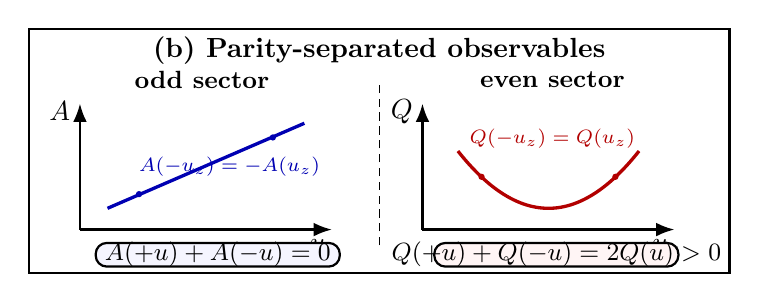
\begin{tikzpicture}[x=1cm,y=1cm,>=Latex]
% =========================================================
% PANEL (b): parity split
% =========================================================
\begin{scope}[shift={(0,-4)}]
  \draw[thick] (0,0) rectangle (8.9,3.1);
  \node[font=\bfseries] at (4.45,2.82) {(b) Parity-separated observables};

  % divider
  \draw[densely dashed] (4.45,0.35) -- (4.45,2.45);

  % left mini-panel odd
  \draw[->, thick] (0.65,0.55) -- (3.85,0.55);
  \draw[->, thick] (0.65,0.55) -- (0.65,2.15);
  \node[below] at (3.75,0.55) {$u_z$};
  \node[left] at (0.65,2.05) {$A$};
  \node[font=\bfseries\small] at (2.2,2.45) {odd sector};

  \draw[blue!70!black, very thick] (1.0,0.82) -- (3.5,1.9);
  \fill[blue!70!black] (1.4,1.0) circle (0.04);
  \fill[blue!70!black] (3.1,1.72) circle (0.04);
  \node[blue!70!black] at (2.55,1.35) {\scriptsize $A(-u_z)=-A(u_z)$};

  \draw[rounded corners, thick, fill=blue!4] (0.85,0.08) rectangle (3.95,0.38);
  \node[align=center, font=\small] at (2.4,0.23) {$A(+u)+A(-u)=0$};

  % right mini-panel even
  \draw[->, thick] (5.0,0.55) -- (8.2,0.55);
  \draw[->, thick] (5.0,0.55) -- (5.0,2.15);
  \node[below] at (8.1,0.55) {$u_z$};
  \node[left] at (5.0,2.05) {$Q$};
  \node[font=\bfseries\small] at (6.65,2.45) {even sector};

  \draw[red!70!black, very thick, smooth, samples=80, domain=-1.15:1.15]
    plot ({6.6+\x},{0.82+0.55*(\x*\x)});
  \fill[red!70!black] (5.75,1.22) circle (0.04);
  \fill[red!70!black] (7.45,1.22) circle (0.04);
  \node[red!70!black] at (6.65,1.7) {\scriptsize $Q(-u_z)=Q(u_z)$};

  \draw[rounded corners, thick, fill=red!4] (5.15,0.08) rectangle (8.25,0.38);
  \node[align=center, font=\small] at (6.7,0.23) {$Q(+u)+Q(-u)=2Q(u)>0$};
\end{scope}

\end{tikzpicture}
\caption{(b) Observable sectors separate by parity under reversal of the signed axial response variable $u_z$: odd signed observables cancel under reversal-symmetric protocols, whereas even scalar observables survive.}
\label{fig:master_overviewB}
\end{figure*}
    
    
    \begin{figure*}[t]
        \centering
        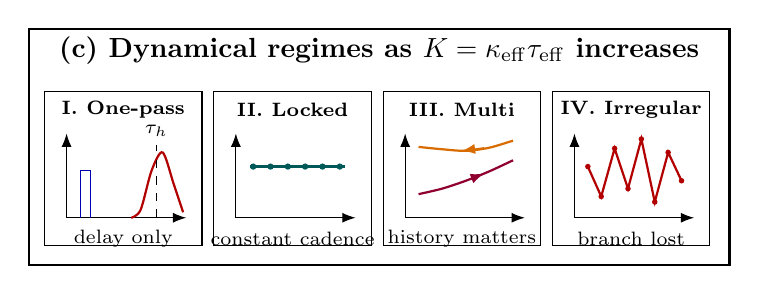
\begin{tikzpicture}[x=1cm,y=1cm,>=Latex]
% =========================================================
% PANEL (c): response regimes
% =========================================================
\begin{scope}[shift={(0,-8)}]
  \draw[thick] (0,0) rectangle (8.9,3.0);
  \node[font=\bfseries] at (4.45,2.72) {(c) Dynamical regimes as $K=\kappa_{\mathrm{eff}}\tau_{\mathrm{eff}}$ increases};

  % Mini panel positions
  % 1
  \begin{scope}[shift={(0.2,0.25)}]
    \draw[thin] (0,0) rectangle (2.0,1.95);
    \node[font=\bfseries\scriptsize] at (1.0,1.72) {I. One-pass};
    \draw[->, thin] (0.28,0.35) -- (1.8,0.35);
    \draw[->, thin] (0.28,0.35) -- (0.28,1.42);
    \draw[thin, blue!70!black] (0.46,0.35) -- (0.46,0.95) -- (0.58,0.95) -- (0.58,0.35);
    \draw[red!70!black, thick, smooth] plot coordinates {(1.10,0.35) (1.22,0.45) (1.36,0.95) (1.50,1.18) (1.64,0.78) (1.76,0.42)};
    \draw[dashed] (1.42,0.35) -- (1.42,1.28);
    \node[font=\scriptsize] at (1.42,1.45) {$\tau_h$};
    \node[font=\scriptsize] at (1.0,0.08) {delay only};
  \end{scope}

  % 2
  \begin{scope}[shift={(2.35,0.25)}]
    \draw[thin] (0,0) rectangle (2.0,1.95);
    \node[font=\bfseries\scriptsize] at (1.0,1.72) {II. Locked};
    \draw[->, thin] (0.28,0.35) -- (1.8,0.35);
    \draw[->, thin] (0.28,0.35) -- (0.28,1.42);
    \foreach \x in {0.5,0.72,0.94,1.16,1.38,1.60} {
      \fill[teal!70!black] (\x,1.0) circle (0.04);
    }
    \draw[teal!70!black, thick] (0.46,1.0) -- (1.66,1.0);
    \node[font=\scriptsize] at (1.0,0.08) {constant cadence};
  \end{scope}

  % 3
  \begin{scope}[shift={(4.5,0.25)}]
    \draw[thin] (0,0) rectangle (2.0,1.95);
    \node[font=\bfseries\scriptsize] at (1.0,1.72) {III. Multi};
    \draw[->, thin] (0.28,0.35) -- (1.8,0.35);
    \draw[->, thin] (0.28,0.35) -- (0.28,1.42);
    \draw[purple!75!black, thick, smooth] plot coordinates {(0.45,0.65) (0.75,0.72) (1.05,0.82) (1.35,0.94) (1.65,1.08)};
    \draw[orange!85!black, thick, smooth] plot coordinates {(0.45,1.25) (0.75,1.22) (1.05,1.20) (1.35,1.24) (1.65,1.33)};
    \draw[->, purple!75!black, thin] (1.0,0.80) -- (1.28,0.91);
    \draw[->, orange!85!black, thin] (1.28,1.24) -- (1.0,1.20);
    \node[font=\scriptsize] at (1.0,0.08) {history matters};
  \end{scope}

  % 4
  \begin{scope}[shift={(6.65,0.25)}]
    \draw[thin] (0,0) rectangle (2.0,1.95);
    \node[font=\bfseries\scriptsize] at (1.0,1.72) {IV. Irregular};
    \draw[->, thin] (0.28,0.35) -- (1.8,0.35);
    \draw[->, thin] (0.28,0.35) -- (0.28,1.42);
    \draw[red!70!black, thick]
      plot coordinates {(0.45,1.00) (0.62,0.62) (0.79,1.23) (0.96,0.72) (1.13,1.35) (1.30,0.55) (1.47,1.18) (1.64,0.82)};
    \foreach \p in {(0.45,1.00),(0.62,0.62),(0.79,1.23),(0.96,0.72),(1.13,1.35),(1.30,0.55),(1.47,1.18),(1.64,0.82)} {
      \fill[red!70!black] \p circle (0.035);
    }
    \node[font=\scriptsize] at (1.0,0.08) {branch lost};
  \end{scope}
\end{scope}

\end{tikzpicture}
\caption{(c) As the effective gain-delay product $K=\kappa_{\mathrm{eff}}\tau_{\mathrm{eff}}$ increases, the platform is expected to pass through one-pass delayed transport, stable locking, multistability, and irregular-response regimes.}
\label{fig:master_overviewC}
\end{figure*}

\section{Governing framework}

\subsection{Rotating-column setting}

Consider an incompressible fluid of density $\rho$ and kinematic viscosity $\nu$ contained in a vertical cylinder of radius $R$ and height $H$. The cylinder rotates with constant angular velocity
\begin{equation}
\bm{\Omega} = \Omega\,\hat{\mathbf z},
\end{equation}
and a compact rotor located near the bottom center provides short, approximately axisymmetric forcing pulses superposed on the slowly rotating base state.

In the rotating frame, the velocity field $\mathbf u(\mathbf x,t)$ and pressure field $p$ satisfy
\begin{equation}
\partial_t \mathbf u + (\mathbf u\cdot \nabla)\mathbf u
+ 2\bm{\Omega}\times \mathbf u
=
-\frac{1}{\rho}\nabla p
+ \nu \nabla^2 \mathbf u
+ \mathbf f,
\label{eq:NSrot}
\end{equation}
together with incompressibility,
\begin{equation}
\nabla\cdot \mathbf u = 0.
\label{eq:incomp}
\end{equation}
Here $\mathbf f(\mathbf x,t)$ denotes the forcing generated by the rotor pulses.

We are interested in the regime
\begin{equation}
\mathrm{Ro}=\frac{U}{2\Omega L}\ll 1,
\qquad
\mathrm{Ek}=\frac{\nu}{\Omega L^2}\ll 1,
\label{eq:RoEk}
\end{equation}
where $U$ and $L$ are characteristic induced speed and length scales. In this regime, the background rotation strongly organizes the response, and the dominant transport is anisotropic rather than isotropically divergent.

\subsection{Axisymmetric vertical forcing and vorticity production}

For axisymmetric forcing, the vertical vorticity
\begin{equation}
\omega_z = (\nabla\times \mathbf u)\cdot \hat{\mathbf z}
\end{equation}
is coupled to the vertical velocity $w=\mathbf u\cdot \hat{\mathbf z}$ through the rotating-fluid dynamics. To leading order, one obtains the rotating-fluid production relation
\begin{equation}
\partial_t \omega_z = 2\Omega\,\partial_z w + \mathcal{R},
\label{eq:vort_vertical}
\end{equation}
where $\mathcal{R}$ collects nonlinear, viscous, and higher-order corrections. Equation~\eqref{eq:vort_vertical} shows that vertical forcing in a rotating medium naturally produces opposite-sign vorticity above and below the forcing region.

This is the first structural point of the experiment: the column is not merely a container for pulses, but a medium whose background rotation transforms vertical forcing into a structured rotational response.

\subsection{Finite axial transport time}

The second structural point is that the response is not instantaneous. When the perturbation projects onto inertial-wave-like modes or other rotation-guided axial response channels, the surface signal appears only after a finite arrival time. In a reduced description, we denote that delay by
\begin{equation}
\tau_h.
\end{equation}

For an idealized inertial-wave packet with wavevector $\mathbf k=(k_r,0,k_z)$ and magnitude $k=\sqrt{k_r^2+k_z^2}$, the rotating-fluid dispersion relation is
\begin{equation}
\omega = 2\Omega \frac{k_z}{k},
\label{eq:inertial_dispersion}
\end{equation}
and the axial group velocity is
\begin{equation}
c_{g,z} = \pdv{\omega}{k_z}.
\end{equation}
Hence the simplest arrival estimate is
\begin{equation}
t_{\mathrm{arr}} \sim \frac{H}{c_{g,z}}.
\label{eq:t_arr}
\end{equation}

For the present paper, the exact microscopic transport channel is less important than the experimentally accessible fact that a reproducible finite delay exists between bottom forcing and surface detection. The measured delay $\tau_h$ is therefore treated as a primary effective parameter of the platform.

\section{Event-defined reinjection loop}

\subsection{From one-pass transport to closed-loop dynamics}

A delayed arrival by itself is only a transport phenomenon. To obtain a genuine delayed nonlinear loop, the detected arrival must be reinjected into the actuation.

Let $t_n^{\mathrm{fire}}$ denote the time at which the $n$th rotor pulse is applied, and let $s(t)$ denote a measured surface observable used for detection. This could be a local surface displacement, optical tracer intensity, pressure fluctuation, or a signed vertical-velocity proxy near the axis.

We define the $n$th detected arrival time by thresholding:
\begin{equation}
t_n^{\mathrm{det}}
=
\inf\left\{
t>t_{n-1}^{\mathrm{fire}}+t_{\mathrm{ref}}
:
s(t)\ge s_{\mathrm{th}}
\right\},
\label{eq:t_detect}
\end{equation}
where $s_{\mathrm{th}}$ is the detection threshold and $t_{\mathrm{ref}}$ is a refractory interval that suppresses multiple triggers from a single arrival or from ringdown.

Each detected event then schedules the next actuation after a fixed digital latency $\tau_d$:
\begin{equation}
t_{n+1}^{\mathrm{fire}} = t_n^{\mathrm{det}} + \tau_d.
\label{eq:t_fire}
\end{equation}

The resulting effective loop delay is
\begin{equation}
\tau_{\mathrm{eff}}
=
\tau_h + \tau_{\mathrm{det}} + \tau_{\mathrm{ctrl}} + \tau_{\mathrm{act}},
\label{eq:tau_eff}
\end{equation}
where the separate terms denote hydrodynamic transport, detector latency, controller latency, and actuation latency.

\subsection{Pulse protocol}

A minimal rotor pulse may be written as
\begin{equation}
P_n(t)=A_n\,\Pi\!\left(\frac{t-t_n^{\mathrm{fire}}}{\Delta t_p}\right),
\label{eq:pulse_def}
\end{equation}
where $A_n$ is the pulse amplitude, $\Delta t_p$ is the pulse width, and $\Pi$ is a rectangular window. More general pulse shapes may be used in practice, but \eqref{eq:pulse_def} is sufficient for reduced modeling.

The simplest feedback prescriptions are
\begin{align}
A_n &= A_0 \qquad \text{(fixed-amplitude reinjection),}
\\
A_{n+1} &= G\,A_n \qquad \text{(gain-controlled reinjection),}
\end{align}
with $G$ an effective feedback gain.

\subsection{Reduced delayed-loop model}

At the fully resolved hydrodynamic level, the reinjected platform is governed by the rotating Navier--Stokes equations together with the event-triggering logic. For analysis, however, it is useful to reduce the loop to an effective phase or response-amplitude description.

Let $\phi(t)$ denote a phase-like variable describing the state of the reinforced axial response. The minimal delay model is then
\begin{equation}
\dot{\phi}(t)
=
\omega_0
+
\kappa_{\mathrm{eff}}
\sin\!\bigl[\phi(t-\tau_{\mathrm{eff}})-\phi(t)\bigr],
\label{eq:reduced_phi}
\end{equation}
where $\omega_0$ is an intrinsic response frequency and $\kappa_{\mathrm{eff}}$ is an effective loop coupling.

Equation~\eqref{eq:reduced_phi} is not presented as an exact derivation from Eqs.~\eqref{eq:NSrot}--\eqref{eq:incomp}. Rather, it is the minimal reduced delayed-loop normal form consistent with event-triggered reinjection and finite transport time. Its role is to organize the experimentally observed branches and their stability.

Uniformly rotating solutions
\begin{equation}
\phi(t)=\Omega_L t + \phi_0
\end{equation}
satisfy the locking condition
\begin{equation}
\Omega_L
=
\omega_0 - \kappa_{\mathrm{eff}}\sin(\Omega_L \tau_{\mathrm{eff}}).
\label{eq:locking_condition}
\end{equation}
Hence finite delay alone can generate multiple candidate branches
\begin{equation}
\Omega_{L,n}
\approx
\frac{2\pi n}{\tau_{\mathrm{eff}}} + \delta\Omega_n,
\qquad n\in\mathbb Z,
\end{equation}
provided the gain-delay product is sufficiently large.

\section{Parity-separated observables}

\subsection{Odd sector}

Let $u_z$ denote a signed axial response coordinate or a signed effective forcing variable. An observable $A$ belongs to the odd sector if
\begin{equation}
A(-u_z) = -A(u_z).
\label{eq:odd_sector}
\end{equation}
Examples include signed angular displacement, signed azimuthal tracer shift, or signed vorticity increment.

In particular, if $\Delta\theta$ denotes a signed angle-like response, then symmetry under reversal of the signed axial episode implies
\begin{equation}
\Delta\theta(+u_z) = -\Delta\theta(-u_z).
\label{eq:theta_odd}
\end{equation}

\subsection{Even sector}

An observable $Q$ belongs to the even sector if
\begin{equation}
Q(-u_z) = Q(u_z).
\label{eq:even_sector}
\end{equation}
Examples include scalar measures quadratic in response speed or swirl intensity, such as
\begin{equation}
Q \propto u_z^2,
\qquad
Q \propto \omega_z^2,
\qquad
Q \propto |X|^2,
\label{eq:Q_examples}
\end{equation}
or cycle-integrated versions thereof.

The point is elementary but powerful:
\begin{equation}
(-u_z)^2=(u_z)^2.
\label{eq:square_even}
\end{equation}
So if one protocol samples both signs of the axial response symmetrically, the even sector is sign-insensitive even when the odd sector is not.

\subsection{Paired-protocol consequence}

Consider a paired forcing protocol generating equal-magnitude opposite-sign response episodes $+u$ and $-u$. Then for odd and even observables one has, respectively,
\begin{align}
A(+u)+A(-u) &= 0,
\label{eq:odd_cancel}
\\
Q(+u)+Q(-u) &= 2Q(u)\ge 0.
\label{eq:even_survive}
\end{align}

Thus a reversal-symmetric protocol can exhibit cancellation in the odd sector while simultaneously exhibiting persistence or accumulation in the even sector.

\begin{proposition}
Let a forcing protocol generate two response episodes with signed amplitudes $+u$ and $-u$, equal duration, and equal magnitude to leading order. If $A$ is odd and $Q$ is even under $u\mapsto -u$, then
\begin{equation}
A(+u)+A(-u)=0,
\qquad
Q(+u)+Q(-u)=2Q(u)\ge 0.
\end{equation}
\end{proposition}

\begin{proof}
Immediate from the defining parity relations.
\end{proof}

This conclusion is purely classical and depends only on parity class, not on any specific microscopic interpretation of the even scalar observable.

\section{Response regimes}

Let
\begin{equation}
K \equiv \kappa_{\mathrm{eff}}\,\tau_{\mathrm{eff}}
\label{eq:Kdef}
\end{equation}
denote the effective gain-delay product. The reduced delayed-loop picture suggests four experimentally distinguishable regimes.

\subsection{Regime I: one-pass delayed transport}

For weak reinjection or no reinjection, the system remains in the transport regime. The key observation is a reproducible delayed arrival at the surface,
\begin{equation}
t_n^{\mathrm{det}} - t_n^{\mathrm{fire}} \approx \tau_h,
\end{equation}
but no stable branch selection occurs.

\subsection{Regime II: stable locking}

At moderate effective gain, repeated event-triggered reinjection reinforces a preferred response cadence. Then one expects
\begin{equation}
t_{n+1}^{\mathrm{det}}-t_n^{\mathrm{det}} \to \text{constant},
\end{equation}
and the pulse-to-pulse response amplitude approaches a stable value
\begin{equation}
X_n \to X_\star.
\end{equation}

\subsection{Regime III: multistability and hysteresis}

For larger $K$, multiple stable response branches may coexist. The experimentally visible signature is that two or more distinct stable operating states exist at the same control parameters, with branch occupancy depending on history, initial preparation, or perturbation.

\subsection{Regime IV: irregular response}

At still larger effective gain or under sufficiently strong nonlinear reinjection, stable locking can break down and the event-interval sequence becomes irregular:
\begin{equation}
\Delta t_n = t_{n+1}^{\mathrm{det}}-t_n^{\mathrm{det}}
\not\to \text{constant}.
\end{equation}
At this stage, the response may become broadband, intermittent, or chaotic in the practical experimental sense.

\section{Experimentally accessible observables and protocol}

A minimal experiment establishing the mechanism described above needs only the following measured quantities:
\begin{enumerate}
\item the one-pass hydrodynamic delay
\begin{equation}
\tau_h = t_{\mathrm{det}}-t_{\mathrm{fire}},
\end{equation}
\item the response amplitude sequence
\begin{equation}
X_n,
\end{equation}
\item the event-interval sequence
\begin{equation}
\Delta t_n = t_{n+1}^{\mathrm{det}}-t_n^{\mathrm{det}},
\end{equation}
\item a signed angle-like response
\begin{equation}
A_n,
\end{equation}
\item an even scalar cycle measure
\begin{equation}
Q_n \propto \int_{t_n}^{t_{n+1}} u^2(t)\,dt
\quad \text{or} \quad
Q_n \propto \int_{t_n}^{t_{n+1}} \omega_z^2(t)\,dt.
\end{equation}
\end{enumerate}

The minimal protocol is:
\begin{enumerate}
\item measure $\tau_h$ without reinjection,
\item verify enhancement of axial coherence under regular pulsing,
\item enable event-triggered reinjection,
\item sweep gain, latency, and background rotation,
\item map locking, multistability, and irregularity,
\item perform paired sign-reversal protocols and compare $A$ with $Q$.
\end{enumerate}

\section{Discussion}

The rotating cylinder with event-triggered reinjection is a classical delayed nonlinear loop. Its interest lies in the fact that the loop is not an abstract delay line, but a rotation-prepared fluid medium with finite transport time and a measurable axial response.

The rotating-fluid part provides the transport channel. The event-triggered reinjection provides the closure. The reduced delayed-loop model provides the branch-selection language. And the parity split provides a clean internal contrast between observables that reverse and observables that do not.

This makes the platform unusually economical. One and the same experiment can demonstrate finite transport delay, reinjection-based branch selection, multistability or irregularity, and the coexistence of cancelling odd observables with persistent even observables.

\section{Conclusion}

We have formulated a classical rotating-fluid platform in which axisymmetric forcing, finite axial transport time, and event-triggered reinjection combine to generate delayed-loop dynamics in a rapidly rotating fluid column.

The central structural result is
\begin{equation}
\text{rotation} + \text{finite transport time} + \text{reinjection}
\Longrightarrow
\text{delayed nonlinear loop behavior}.
\end{equation}
Within this loop, parity separates the observable space into two distinct sectors:
\begin{equation}
A(-u_z)=-A(u_z),
\qquad
Q(-u_z)=Q(u_z).
\end{equation}
Hence reversal-symmetric forcing can yield leading-order cancellation in a signed angle-like observable while preserving a nonzero scalar contribution in the even sector.

No quantum assumptions are required for any part of this argument. The result is entirely classical and rests only on rotating-fluid transport, event-defined reinjection, delay-induced selection structure, and parity.

\appendix

\section{Compact reduced notation}

For convenience, the main reduced parameters are
\begin{align}
\tau_{\mathrm{eff}}
&=
\tau_h + \tau_{\mathrm{det}} + \tau_{\mathrm{ctrl}} + \tau_{\mathrm{act}},
\\
K
&=
\kappa_{\mathrm{eff}}\,\tau_{\mathrm{eff}},
\\
t_n^{\mathrm{det}}
&=
\inf\left\{
t>t_{n-1}^{\mathrm{fire}}+t_{\mathrm{ref}}
:
s(t)\ge s_{\mathrm{th}}
\right\},
\\
t_{n+1}^{\mathrm{fire}}
&=
t_n^{\mathrm{det}}+\tau_d.
\end{align}

\begin{thebibliography}{99}

\bibitem{Greenspan1968}
H.~P.~Greenspan,
1968,
\emph{The Theory of Rotating Fluids},
Cambridge University Press, Cambridge.

\bibitem{Batchelor1967}
G.~K.~Batchelor,
1967,
\emph{An Introduction to Fluid Dynamics},
Cambridge University Press, Cambridge.

\bibitem{Pedlosky1987}
J.~Pedlosky,
1987,
\emph{Geophysical Fluid Dynamics},
2nd ed.,
Springer, New York.

\bibitem{YeungStrogatz1999}
M.~K.~S.~Yeung and S.~H.~Strogatz,
1999,
``Time delay in the Kuramoto model of coupled oscillators,''
\emph{Physical Review Letters}
\textbf{82}(3), 648--651,
DOI: 10.1103/PhysRevLett.82.648.

\bibitem{YanchukGiacomelli2017}
S.~Yanchuk and G.~Giacomelli,
2017,
``Spatio-temporal phenomena in complex systems with time delays,''
\emph{Journal of Physics A: Mathematical and Theoretical}
\textbf{50}(10), 103001,
DOI: 10.1088/1751-8121/aa5e8c.

\bibitem{Willis2012}
J.~R.~Willis,
2012,
``The construction of effective relations for waves in a composite,''
\emph{Comptes Rendus M\'ecanique}
\textbf{340}(4--5), 181--192,
DOI: 10.1016/j.crme.2012.02.006.

\bibitem{Iskandarani2026SST55}
O.~Iskandarani,
2026,
``Delay-Induced Mode Selection in Circulating Feedback Systems,''
manuscript under review at \emph{AIP Advances}.

\bibitem{Iskandarani2026SST46}
O.~Iskandarani,
2026,
``Relational Time-of-Arrival as a Covariant Field Observable: From Event Currents to a Continuum Clock Limit,''
preprint / manuscript.

\bibitem{Iskandarani2026VAM1772}
O.~Iskandarani,
2026,
``Reversible Azimuthal Response to Axisymmetric Vertical Forcing in Rapidly Rotating Fluids,''
unpublished manuscript draft (VAM-17.7.2).

\bibitem{Iskandarani2026VAM178}
O.~Iskandarani,
2026,
``Impulsive Bottom-Rotor Forcing, Delayed Surface Response, and Event-Triggered Reinjection in a Rotating Fluid Column,''
unpublished manuscript draft (VAM-17.8).

\end{thebibliography}

\end{document}